%!TEX root =../../course-notes.tex
% ^ leave for LaTeXTools build functionality

\begin{module}{Module E: Solving Systems of Linear Equations}

\begin{moduleStandards}
  \item \textbf{E1: Systems as matrices.}
        Translate back and forth between a system of linear equations and
        the corresponding augmented matrix.
  \item \textbf{E2: Row reduction.}
        Put a matrix in reduced row echelon form
  \item \textbf{E3: Solving Linear Systems.}
        Solve a system of linear equations.
  \item \textbf{E4: Homogeneous Systems.}
        Find a basis for the solution set of a homogeneous linear system.
\end{moduleStandards}

%!TEX root =../../course-notes.tex
% ^ leave for LaTeXTools build functionality

\newcommand{\systemWithOneSolutionA}{
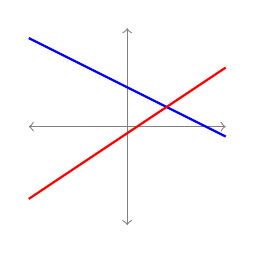
\begin{tikzpicture}[scale=0.25]
\draw[thin,gray,<->] (-5,0) -- (5,0);
\draw[thin,gray,<->] (0,-5) -- (0,5);
\draw[thick,blue] (-5,4.5) -- (5,-0.5);
\draw[thick,red] (-5,-3.67) -- (5,3);
\end{tikzpicture}
}

\newcommand{\systemWithOneSolutionB}{
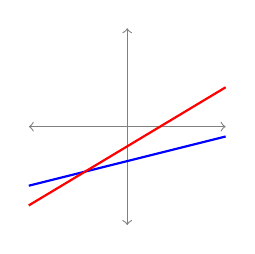
\begin{tikzpicture}[scale=0.25]
\draw[thin,gray,<->] (-5,0) -- (5,0);
\draw[thin,gray,<->] (0,-5) -- (0,5);
\draw[thick,blue] (-5,-3) -- (5,-0.5);
\draw[thick,red] (-5,-4) -- (5,2);
\end{tikzpicture}
}

\newcommand{\systemWithInfinitelyManySolutions}{
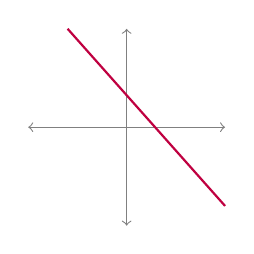
\begin{tikzpicture}[scale=0.25]
\draw[thin,gray,<->] (-5,0) -- (5,0);
\draw[thin,gray,<->] (0,-5) -- (0,5);
\draw[thick,purple] (-3,5) -- (5,-4);
\end{tikzpicture}
}

\newcommand{\systemWithNoSolutions}{
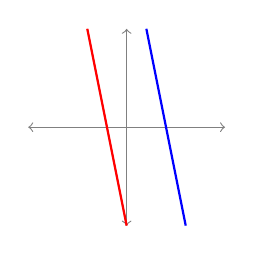
\begin{tikzpicture}[scale=0.25]
\draw[thin,gray,<->] (-5,0) -- (5,0);
\draw[thin,gray,<->] (0,-5) -- (0,5);
\draw[thick,blue] (3,-5) -- (1,5);
\draw[thick,red] (0,-5) -- (-2,5);
\end{tikzpicture}
}

%!TEX root =../../course-notes.tex
% ^ leave for LaTeXTools build functionality


\begin{readinessAssuranceOutcomes}
\item Determine if a system to a two-variable system of linear equations
      will have zero, one, or infinitely-many solutions by graphing.
\item Find the unique solution to a two-variable system of linear equations
      by back-substitution.
\end{readinessAssuranceOutcomes}

\begin{readinessAssuranceResources}
\item \url{https://www.khanacademy.org/math/cc-eighth-grade-math/cc-8th-systems-topic/cc-8th-systems-graphically/a/systems-of-equations-with-graphing}
\item \url{https://www.khanacademy.org/math/algebra/systems-of-linear-equations/solving-systems-of-equations-with-substitution/v/practice-using-substitution-for-systems}
\end{readinessAssuranceResources}


%Form B005 Answer key, problems 1-10
%1  C
%2  A
%3  D
%4  D
%5  B
%6  A
%7  A
%8  C
%9  D
%10 B

\begin{readinessAssuranceTest}
%1  C
\item Which of these graphs represents the following system of linear equations?
      \begin{align*}
      x+2y   &=   4 \\
      2x-3y  &=  1
      \end{align*}

\begin{multicols}{4}
\begin{readinessAssuranceTestChoices}
\item \systemWithInfinitelyManySolutions
\item \systemWithNoSolutions
\item \systemWithOneSolutionA % correct
\item \systemWithOneSolutionB
\end{readinessAssuranceTestChoices}
\end{multicols}


%2  A
\item How many solutions are there for the system of linear equations
      represented by the following graph?
    \begin{center}
      \systemWithOneSolutionB
    \end{center}

\begin{multicols}{4}
\begin{readinessAssuranceTestChoices}
\item One % correct
\item Two
\item Zero
\item Infinitely-many
\end{readinessAssuranceTestChoices}
\end{multicols}

%3  D
\item Which of these graphs represents the following system of linear equations?
      \begin{align*}
      3x+3y   &=   6 \\
      x+y  &=  2
      \end{align*}

\begin{multicols}{4}
\begin{readinessAssuranceTestChoices}
\item \systemWithOneSolutionA
\item \systemWithOneSolutionB
\item \systemWithNoSolutions
\item \systemWithInfinitelyManySolutions % correct
\end{readinessAssuranceTestChoices}
\end{multicols}



%4  D
\item How many solutions are there for the system of linear equations
      represented by the following graph? (This graph represents two completely
      overlapping lines.)
    \begin{center}
      \systemWithInfinitelyManySolutions
    \end{center}

\begin{multicols}{4}
\begin{readinessAssuranceTestChoices}
\item Zero
\item One
\item Two
\item Infinitely-many % correct
\end{readinessAssuranceTestChoices}
\end{multicols}


%5  B
\item How many solutions are there for the system of linear equations
      represented by the following graph?
    \begin{center}
      \systemWithOneSolutionA
    \end{center}

\begin{multicols}{4}
\begin{readinessAssuranceTestChoices}
\item Zero
\item One % correct
\item Two
\item Infinitely-many
\end{readinessAssuranceTestChoices}
\end{multicols}


%6  A
\item How many solutions are there for the system of linear equations
      represented by the following graph? (This graph represents two
      non-overlapping parallel lines.)
    \begin{center}
      \systemWithNoSolutions
    \end{center}

\begin{multicols}{4}
\begin{readinessAssuranceTestChoices}
\item Zero % correct
\item One
\item Two
\item Infinitely-many
\end{readinessAssuranceTestChoices}
\end{multicols}


%7  A
\item Solve the following system of linear equations.
      \begin{align*}
      y   &=   2x+5 \\
      y  &=  -x+2
      \end{align*}

\begin{multicols}{4}
\begin{readinessAssuranceTestChoices}
\item \((x,y)=(-1,3)\) % correct
\item \((x,y)=(4,-2)\)
\item There are no solutions.
\item There are infinitely-many solutions.
\end{readinessAssuranceTestChoices}
\end{multicols}


%8  C
\item Solve the following system of linear equations.
      \begin{align*}
      y   &=  3x+5 \\
      y  &=  3x+2
      \end{align*}

\begin{multicols}{4}
\begin{readinessAssuranceTestChoices}
\item
\((x,y)=(3,4)\)
\item
\((x,y)=(-5,1)\)
\item There are no solutions. % correct
\item There are infinitely-many solutions.
\end{readinessAssuranceTestChoices}
\end{multicols}


%9  D
\item Solve the following system of linear equations.
      \begin{align*}
      x+2y   &=   4 \\
      2x-3y  &=  1
      \end{align*}

\begin{multicols}{4}
\begin{readinessAssuranceTestChoices}
\item There are no solutions.
\item There are infinitely-many solutions.
\item
\((x,y)=(-1,4)\)
\item
\((x,y)=(2,1)\) % correct
\end{readinessAssuranceTestChoices}
\end{multicols}


%10 B
\item Solve the following system of linear equations.
      \begin{align*}
      4x-8y   &= 12 \\
      -6x+12y  &=  18
      \end{align*}

\begin{multicols}{4}
\begin{readinessAssuranceTestChoices}
\item There are no solutions.
\item There are infinitely-many solutions. % correct
\item
\((x,y)=(3,3)\)
\item
\((x,y)=(-2,1)\)
\end{readinessAssuranceTestChoices}
\end{multicols}

\end{readinessAssuranceTest}

%!TEX root =../../course-notes.tex
% ^ leave for LaTeXTools build functionality

\begin{applicationActivities}{1}{4}

\begin{definition}
A \term{linear equation} is an equation of the variables \(x_i\) of the form
\[
a_1x_1+a_2x_2+\dots+a_nx_n=b
.\]
A \term{solution}
for a linear equation is expressed in terms of the Euclidean vectors
\[
  \begin{bmatrix}
    x_1 \\
    x_2 \\
    \vdots \\
    x_n
  \end{bmatrix}=
  \begin{bmatrix}
    s_1 \\
    s_2 \\
    \vdots \\
    s_n
  \end{bmatrix}
\]
and must satisfy
\[
a_1s_1+a_2s_2+\dots+a_ns_n=b
.\]
\end{definition}

\begin{observation}
The linear equation \(3x-5y=-2\) may be graphed as a line in the \(xy\) plane.

\begin{center}
\begin{tikzpicture}[scale=0.3]
\draw[thin,gray,<->] (-5,0) -- (5,0);
\draw[thin,gray,<->] (0,-5) -- (0,5);
\draw[thick,blue] (-5,-2.6) -- (5,3.4);
% \draw[thick,red] (-5,-3.67) -- (5,3);
\end{tikzpicture}
\end{center}

The linear equation \(x+2y-z=4\) may be graphed as a plane in \(xyz\) space.
\end{observation}

\begin{remark}
In previous classes you likely assumed \(x=x_1\), \(y=x_2\), and \(z=x_3\).
However, since this course often deals with equations of four or more
variables, we will almost always write our variables as \(x_i\).
\end{remark}

\begin{definition}
A \term{system of linear equations} (or a \term{linear system} for short)
is a collection of one or more linear equations.
  \begin{alignat*}{5}
    a_{11}x_1 &\,+\,& a_{12}x_2 &\,+\,& \dots  &\,+\,& a_{1n}x_n &\,=\,& b_1 \\
    a_{21}x_1 &\,+\,& a_{22}x_2 &\,+\,& \dots  &\,+\,& a_{2n}x_n &\,=\,& b_2 \\
     \vdots&  &\vdots&   &&  &\vdots&&\vdots  \\
    a_{m1}x_1 &\,+\,& a_{m2}x_2 &\,+\,& \dots  &\,+\,& a_{mn}x_n &\,=\,& b_m
  \end{alignat*}
A \term{solution}
\[
  \begin{bmatrix}
    x_1 \\
    x_2 \\
    \vdots \\
    x_n
  \end{bmatrix}=
  \begin{bmatrix}
    s_1 \\
    s_2 \\
    \vdots \\
    s_n
  \end{bmatrix}
\]
for a linear system satisfies
\[
a_{i1}s_1+a_{i2}s_2+\dots+a_{in}s_n=b_i
\]
for \(1\leq i\leq m\) (that is, the solution satisfies all equations
in the system).
\end{definition}

\begin{remark}
  When variables in a large linear system are missing, we prefer to
  write the system in one of the following standard forms:

  \begin{multicols}{3}\noindent
    Original linear system:
    \begin{alignat*}{2}
       x_1 + 3x_3 &\,=\,& 3 \\
      3x_1 - 2x_2 + 4x_3 &\,=\,& 0 \\
      -x_2 +  x_3 &\,=\,& -2
    \end{alignat*}
    Verbose standard form:
    \begin{alignat*}{4}
       x_1 &\,+\,& 0x_2 &\,+\,& 3x_3 &\,=\,& 3 \\
      3x_1 &\,-\,& 2x_2 &\,+\,& 4x_3 &\,=\,& 0 \\
      0x_1 &\,-\,&  x_2 &\,+\,&  x_3 &\,=\,& -2
    \end{alignat*}
    Concise standard form:
    \begin{alignat*}{4}
       x_1 &     &      &\,+\,& 3x_3 &\,=\,& 3 \\
      3x_1 &\,-\,& 2x_2 &\,+\,& 4x_3 &\,=\,& 0 \\
           &\,-\,&  x_2 &\,+\,&  x_3 &\,=\,& -2
    \end{alignat*}
  \end{multicols}
\end{remark}

\begin{definition}
  A linear system is \term{consistent} if there exists a solution for the
  system. Otherwise it is \term{inconsistent}.
\end{definition}

\begin{fact}
  All linear systems are either \textbf{consistent with one solution},
  \textbf{consistent with infinitely-many solutions}, or
  \textbf{inconsistent}.
\end{fact}

\begin{activity}{5}
  Consider the following graphs representing linear systems of two variables.
  Label each graph with \textbf{consistent with one solution},
  \textbf{consistent with infinitely-many solutions}, or
  \textbf{inconsistent}.
  \begin{multicols}{4}
  \begin{center}
    \systemWithInfinitelyManySolutions
    \systemWithOneSolutionB
    \systemWithNoSolutions
    \systemWithOneSolutionA
  \end{center}
  \end{multicols}
\end{activity}

\begin{activity}{10}
  All inconsistent linear systems contain a logical \term{contradiction}.
  Find a contradiction in this system.
  \begin{align*}
  -x_1+2x_2  &=  5 \\
  2x_1-4x_2  &=  6
  \end{align*}
\end{activity}

\begin{activity}{10}
  Consider the following consistent linear system.
  \begin{align*}
  -x_1+2x_2  &= -3 \\
  2x_1-4x_2  &=  6
  \end{align*}
\begin{subactivity}
  Find three different solutions
  \(
    \begin{bmatrix}
      x_1 \\
      x_2
    \end{bmatrix}=
    \begin{bmatrix}
      r_1 \\
      r_2
    \end{bmatrix},
    \begin{bmatrix}
      s_1 \\
      s_2
    \end{bmatrix},
    \begin{bmatrix}
      t_1 \\
      t_2
    \end{bmatrix}
  \)
  for this system.
\end{subactivity}
\begin{subactivity}
  Let \(x_2=a\) where \(a\) is an arbitrary real number, then find an
  expression for \(x_1\) in terms of \(a\). Use this to describe \textit{all}
  solutions (the \term{solution set})
  \(
    \begin{bmatrix}
      x_1 \\
      x_2
    \end{bmatrix}=
    \begin{bmatrix}
      ? \\
      a
    \end{bmatrix}
  \)
  for the linear system in terms of \(a\).
\end{subactivity}
\end{activity}

% \begin{remark}
%   The solution set of a consistent linear system with infinitely many solutions
%   may be described by setting each
%   certain variable equal to an arbitrary parameter, and expressing the
%   other variables in terms of those parameters. (Later we will learn
%   how to do this methodically.)
% \end{remark}

\begin{activity}{10}
  Consider the following linear system.
  \begin{alignat*}{5}
    x_1 &\,+\,& 2x_2 &\, \,&     &\,-\,&  x_4 &\,=\,& 3 \\
        &\, \,&      &\, \,& x_3 &\,+\,& 4x_4 &\,=\,& -2
  \end{alignat*}
  Describe the solution set
  \[
    \begin{bmatrix}
      x_1 \\
      x_2 \\
      x_3 \\
      x_4
    \end{bmatrix}=
    \begin{bmatrix}
      ? \\
      a \\
      ? \\
      b
    \end{bmatrix}=
    \begin{bmatrix}
      t_1 \\
      0 \\
      t_3 \\
      0
    \end{bmatrix}+
    a\begin{bmatrix}
      ? \\
      1 \\
      ? \\
      0
    \end{bmatrix}+
    b\begin{bmatrix}
      ? \\
      0 \\
      ? \\
      1
    \end{bmatrix}
  \] to the linear system
  by setting \(x_2=a\) and \(x_4=b\), and then solving for \(x_1\) and
  \(x_3\).
\end{activity}

\begin{observation}
  Solving linear systems of two variables by graphing or substitution is
  reasonable for two-variable systems, but these simple techniques
  won't cut it for equations with
  more than two variables or more than two equations.
\end{observation}

\begin{remark}
  The only important information in a linear system are its coefficients and
  constants.

  \begin{multicols}{3}\noindent
    Original linear system:
    \begin{alignat*}{2}
       x_1 + 3x_3 &\,=\,& 3 \\
      3x_1 - 2x_2 + 4x_3 &\,=\,& 0 \\
      -x_2 +  x_3 &\,=\,& -2
    \end{alignat*}
    Verbose standard form:
    \begin{alignat*}{4}
       x_1 &\,+\,& 0x_2 &\,+\,& 3x_3 &\,=\,& 3 \\
      3x_1 &\,-\,& 2x_2 &\,+\,& 4x_3 &\,=\,& 0 \\
      0x_1 &\,-\,&  x_2 &\,+\,&  x_3 &\,=\,& -2
    \end{alignat*}
    Coefficients/constants:
    \begin{alignat*}{4}
       1 &     &  0 &\,\,& 3 &\,|\,& 3 \\
       3 &\, \,& -2 &\,\,& 4 &\,|\,& 0 \\
       0 &\, \,&  1 &\,\,& 1 &\,|\,& -2
    \end{alignat*}
  \end{multicols}
\end{remark}

\begin{definition}
  A system of \(m\) linear equations with \(n\) variables is often represented
  by writing its coefficients and constants in an \term{augmented matrix}.
  \begin{multicols}{2}\noindent
  \begin{alignat*}{5}
    a_{11}x_1 &\,+\,& a_{12}x_2 &\,+\,& \dots  &\,+\,& a_{1n}x_n &\,=\,& b_1 \\
    a_{21}x_1 &\,+\,& a_{22}x_2 &\,+\,& \dots  &\,+\,& a_{2n}x_n &\,=\,& b_2 \\
     \vdots&  &\vdots&   &&  &\vdots&&\vdots  \\
    a_{m1}x_1 &\,+\,& a_{m2}x_2 &\,+\,& \dots  &\,+\,& a_{mn}x_n &\,=\,& b_m
  \end{alignat*}
  \[
    \begin{bmatrix}[cccc|c]
      a_{11} & a_{12} & \cdots & a_{1n} & b_1\\
      a_{21} & a_{22} & \cdots & a_{2n} & b_2\\
      \vdots & \vdots & \ddots & \vdots & \vdots\\
      a_{m1} & a_{m2} & \cdots & a_{mn} & b_m
    \end{bmatrix}
  \]
  \end{multicols}
\end{definition}

\begin{definition}
  Two systems of linear equations (and their corresponding augmented
  matrices) are said to be \term{equivalent} if they have the same
  solution set.
\end{definition}

\begin{activity}{10}
  Following are six procedures used to manipulate an augmented matrix.
  Label the procedures that would result in an equivalent augmented
  matrix as \textbf{valid}, and label the procedures that would
  change the solution set of the corresponding linear system as
  \textbf{invalid}.
  \begin{multicols}{2}
    \begin{enumerate}[a)]
      \item Swap two rows.
      \item Swap two columns.
      \item Add a constant to every term in a row.
      \item Multiply a row by a conzero constant.
      \item Add a constant multiple of one row to another row.
      \item Replace a column with zeros.
    \end{enumerate}
  \end{multicols}
  \begin{TBLnote}
    This activity could be ran as a card sort.
  \end{TBLnote}
\end{activity}

\end{applicationActivities}

%!TEX root =../../course-notes.tex
% ^ leave for LaTeXTools build functionality

\begin{applicationActivities}{2}{4}

\begin{fact}
  Every augmented matrix \(A\) reduces to a unique reduced row echelon form
  matrix. This matrix is denoted as \(\RREF(A)\).
\end{fact}

\begin{activity}{10}
  Consider the following matrix.
  \[
    A = \begin{bmatrix}[ccc|c]
      1 & 2 & 3 & 1\\
      2 & 4 & 8 & 0
    \end{bmatrix}
  \]
  \begin{subactivity}
    Find \(\RREF(A)\) (Use CoCalc).
  \end{subactivity}
  \begin{subactivity}
    How many solutions does the corresponding linear system have?
  \end{subactivity}
\end{activity}

\begin{activity}{10}
Consider the (simpler) system from the previous problem:
	\begin{alignat*}{3}
		x_1 &+ 2x_2 & &= 4\\
	     	 & &x_3 &= -1
	\end{alignat*}
\begin{subactivity}
Let $x_1=a$ and write the solution set in the form 
\( \left\{ \begin{bmatrix} a \\ ? \\ ? \end{bmatrix} \,\middle|\, a \in \IR \right\} \)
\end{subactivity}
\begin{subactivity}
Let $x_2=b$ and write the solution set in the form 
\( \left\{ \begin{bmatrix} ? \\ b \\ ? \end{bmatrix} \,\middle|\, b \in \IR \right\} \)
\end{subactivity}
\begin{subactivity}
Which of these was easier?  What features of the RREF matrix \[\begin{bmatrix}[ccc|c] 1 & 2 & 0 & 4 \\ 0 & 0 & 1 & -1 \end{bmatrix}\] cause this?
\end{subactivity}
\end{activity}

\begin{definition}
If a matrix is in reduced row echelon form, a \term{pivot} is an entry satisfying
\begin{enumerate}[1.]
\item It is $1$
\item Everything else in the same row but to the left of it is zero
\item Everything else in the same column is zero.
\end{enumerate}

For example, the pivots are circled in 

\[\begin{bmatrix}[ccc|c] \circledNumber{1} & 2 & 0 & 4 \\ 0 & 0 & \circledNumber{1} & -1 \end{bmatrix}\]
\end{definition}


\begin{activity}{5}
Circle the pivots in each matrix below.
\begin{multicols}{2}
\[ \begin{bmatrix}[cccc|c] 1 & 1 & 0 & 0 & 2 \\ 0 & 0 & 1 & 0 &  0 \\ 0 & 0 & 0 &  1 & 1 \end{bmatrix} \]
\[ \begin{bmatrix}[cccc|c] 1 & 1 & 0 & 1 & 0 \\ 0 & 0 & 1 & 1 & 0 \\ 0 & 0 & 0 & 0  & 0 \end{bmatrix} \]
\[ \begin{bmatrix}[ccc|c] 1 & 0 & 1 & 2 \\ 0 & 1 & 0 & 1 \end{bmatrix} \]
\[ \begin{bmatrix}[ccc|c] 1 & 0 & 0 & 2 \\ 0 & 1 & 1 & 0 \\ 0 & 0 & 0 & 0 \end{bmatrix} \]
\end{multicols}
\end{activity}


\end{applicationActivities}

%!TEX root =../../course-notes.tex
% ^ leave for LaTeXTools build functionality

\begin{applicationActivities}{3}{5}

\begin{definition}
  An algorithm that reduces \(A\) to \(\RREF(A)\) is called
  \term{Gauss-Jordan elimination}. For example:
  \begin{multicols}{3}
    \begin{enumerate}
      \item Circle the top-left-most cell that (a) is below any existing pivot
      positions and (b) has a nonzero term either in that position or below it.
      \item Ignoring any rows above this pivot position, use row operations
      to change the value of your pivot position to \(1\), and the terms below
      it to \(0\).
      \item Repeat these two steps as often as possible.
      \item Finally,
      zero out any terms above pivot positions.
    \end{enumerate}
  \end{multicols}
\end{definition}

\begin{observation}
  Here is an example of applying Gauss-Jordan elimination to a matrix:
  \[
    \begin{bmatrix}[ccc|c]
      \circledNumber{3} & -2 & 13 & 6 \\
      2 & -2 & 10 & 2 \\
      -1 & 3 & -6 & 11
    \end{bmatrix}\sim
    \begin{bmatrix}[ccc|c]
     \circledNumber{2} & -2 & 10 & 2 \\
      3 & -2 & 13 & 6 \\
      -1 & 3 & -6 & 11
    \end{bmatrix}\sim
    \begin{bmatrix}[ccc|c]
     \circledNumber{1} & -1 & 5 & 1 \\
      3 & -2 & 13 & 6 \\
      -1 & 3 & -6 & 11
    \end{bmatrix}
  \]
  \[\sim
    \begin{bmatrix}[ccc|c]
     \circledNumber{1} & -1 & 5 & 1 \\
      0 & \circledNumber{1} & -2 & 3 \\
      0 & 2 & -1 & 12
    \end{bmatrix}
    \sim
      \begin{bmatrix}[ccc|c]
       \circledNumber{1} & -1 & 5 & 1 \\
        0 & \circledNumber{1} & -2 & 3 \\
        0 & 0 & \circledNumber{3} & 6
      \end{bmatrix}
    \sim
    \begin{bmatrix}[ccc|c]
     \circledNumber{1} & -1 & 5 & 1 \\
      0 & \circledNumber{1} & -2 & 3 \\
      0 & 0 & \circledNumber{1} & 2
    \end{bmatrix}
  \]
  \[\sim
    \begin{bmatrix}[ccc|c]
     \circledNumber{1} & -1 & 5 & 1 \\
      0 & \circledNumber{1} & -2 & 3 \\
      0 & 0 & \circledNumber{1} & 2
    \end{bmatrix}
    \sim
    \begin{bmatrix}[ccc|c]
     \circledNumber{1} & -1 & 0 & -9 \\
      0 & \circledNumber{1} & 0 & 7 \\
      0 & 0 & \circledNumber{1} & 2
    \end{bmatrix}
    \sim
    \begin{bmatrix}[ccc|c]
     \circledNumber{1} & 0 & 0 & -2 \\
      0 & \circledNumber{1} & 0 & 7 \\
      0 & 0 & \circledNumber{1} & 2
    \end{bmatrix}
  \]
\end{observation}

\begin{activity}{15}
  Find \(\RREF(A)\) where
  \[A=
    \begin{bmatrix}[cccc|c]
      -1 &  1 & -3 &  2 &  0 \\
       2 & -1 &  5 &  3 & -11 \\
       3 &  2 &  4 &  1 &  1 \\
       0 &  1 & -1 &  1 &  1 \\
    \end{bmatrix}
  .\]
\end{activity}

\begin{definition}
  The columns of \(\RREF(A)\) without a leading term represent
  \term{free variables} of the linear system modeled by \(A\)
  that may be set equal to arbitrary parameters.
  The other \term{bounded variables} can then be expressed in terms
  of those parameters to describe the solution set
  to the linear system modeled by \(A\).
\end{definition}

\begin{activity}{10}
  Given the linear system and its equivalent row-reduced matrix
  \begin{multicols}{2}\noindent
    \begin{alignat*}{5}
      -x_1 &\,+\,&  x_2 &\,-\,&  3x_3 &\,+\,&  2x_4 &\,=\,& 0 \\
      2x_1 &\,-\,&  x_2 &\,+\,&  5x_3 &\,+\,&  3x_4 &\,=\,& -11 \\
      3x_1 &\,+\,& 2x_2 &\,+\,&  4x_3 &\,+\,&   x_4 &\,=\,& 1 \\
           &\, \,&  x_2 &\,-\,&   x_3 &\,+\,&   x_4 &\,=\,& 1 \\
    \end{alignat*}
  \[
    \begin{bmatrix}[cccc|c]
       1 &  0 &  2 &  0 & -1 \\
       0 &  1 & -1 &  0 &  3 \\
       0 &  0 &  0 &  1 & -2 \\
       0 &  0 &  0 &  0 &  0 \\
    \end{bmatrix}
  \]
  \end{multicols}
  circle the pivot positions and describe the solution set
  \(
    \begin{bmatrix}
      x_1 \\
      x_2 \\
      x_3 \\
      x_4
    \end{bmatrix}=
    \begin{bmatrix}
      p_1 \\
      p_2 \\
      p_3 \\
      p_4
    \end{bmatrix}
    +a\begin{bmatrix}
      s_1 \\
      s_2 \\
      s_3 \\
      s_4
    \end{bmatrix}
  \) by setting the free variable (the column without a pivot position)
  equal to \(a\), and expressing each of the other
  bounded variables equal to an expression in terms of \(a\).
\end{activity}

\begin{remark}
  It's not necessary to completely find \(\RREF(A)\) to
  deduce that a linear system is inconsistent.
\end{remark}

\begin{activity}{10} %TODO remove matrices, focus on augmented matrix
  Find a contradiction in the inconsistent linear system
    \begin{alignat*}{4}
      2x_1 &\,-\,& 3x_2 &\,=\,& 17 \\
       x_1 &\,+\,& 2x_2 &\,=\,& -2 \\
      -x_1 &\,-\,&  x_2 &\,=\,& 1
    \end{alignat*}
  by considering the following equivalent augmented matrices:
  \[
    \begin{bmatrix}[cc|c]
       2 & -3 & 17 \\
       1 &  2 & -2 \\
      -1 & -1 &  1 \\
    \end{bmatrix}\sim
    \begin{bmatrix}[cc|c]
       1 &  2 & -2 \\
       0 &  1 &  3 \\
       0 &  0 &  2 \\
    \end{bmatrix}
  .\]
\end{activity}

\begin{activity}{5}
  Show that all linear systems of the form
  \begin{alignat*}{5}
    a_{11}x_1 &\,+\,& a_{12}x_2 &\,+\,& \dots  &\,+\,& a_{1n}x_n &\,=\,& 0 \\
    a_{21}x_1 &\,+\,& a_{22}x_2 &\,+\,& \dots  &\,+\,& a_{2n}x_n &\,=\,& 0 \\
     \vdots&  &\vdots&   &&  &\vdots&&\vdots  \\
    a_{m1}x_1 &\,+\,& a_{m2}x_2 &\,+\,& \dots  &\,+\,& a_{mn}x_n &\,=\,& 0
  \end{alignat*}
  are consistent by finding a
  quickly verifiable solution.
\end{activity}

\begin{definition}
  A \term{homogeneous system} is a linear system satisfying \(b_i=0\), that is,
  it is a linear system of the form
  \begin{alignat*}{5}
    a_{11}x_1 &\,+\,& a_{12}x_2 &\,+\,& \dots  &\,+\,& a_{1n}x_n &\,=\,& 0 \\
    a_{21}x_1 &\,+\,& a_{22}x_2 &\,+\,& \dots  &\,+\,& a_{2n}x_n &\,=\,& 0 \\
     \vdots&  &\vdots&   &&  &\vdots&&\vdots  \\
    a_{m1}x_1 &\,+\,& a_{m2}x_2 &\,+\,& \dots  &\,+\,& a_{mn}x_n &\,=\,& 0
  \end{alignat*}
\end{definition}

\begin{fact}
  Because the zero vector is always a solution,
  the solution set to any homogeneous system with infinitely-many solutions
  may be generated by multiplying the parameters representing the free variables
  by a minimal set of Euclidean vectors, and adding these up. For example:
  \[
    \begin{bmatrix}
      x_1 \\
      x_2 \\
      x_3 \\
      x_4
    \end{bmatrix}=
    a\begin{bmatrix}
      3 \\
      1 \\
      -1 \\
      0
    \end{bmatrix}+
    b\begin{bmatrix}
      0 \\
      0 \\
      0 \\
      1
    \end{bmatrix}
  \]
\end{fact}

\begin{definition}
  A minimal set of Euclidean vectors generating the solution set to a
  homogeneous system is called a \textbf{basis} for the solution
  set of the homogeneous system. For example:
  \begin{multicols}{2}\noindent
  \[
    \begin{bmatrix}
      x_1 \\
      x_2 \\
      x_3 \\
      x_4
    \end{bmatrix}=
    a\begin{bmatrix}
      3 \\
      1 \\
      -1 \\
      0
    \end{bmatrix}+
    b\begin{bmatrix}
      0 \\
      0 \\
      0 \\
      1
    \end{bmatrix}
  \]
  \[
    \textrm{Basis}=\left\{
    \begin{bmatrix}
      3 \\
      1 \\
      -1 \\
      0
    \end{bmatrix},
    \begin{bmatrix}
      0 \\
      0 \\
      0 \\
      1
    \end{bmatrix}\right\}
  \]
  \end{multicols}
\end{definition}

\begin{activity}{10}
  Find a basis for the solution set of the following homogeneous linear
  system.
  \begin{alignat*}{5}
    x_1 &\,+\,& 2x_2 &\, \,&     &\,-\,&  x_4 &\,=\,& 0 \\
        &\, \,&      &\, \,& x_3 &\,+\,& 4x_4 &\,=\,& 0 \\
   2x_1 &\,+\,& 4x_2 &\,+\,& x_3 &\,+\,& 2x_4 &\,=\,& 0 \\
  \end{alignat*}
\end{activity}




\end{applicationActivities}


\end{module}
